\chapter[~~~CONCEPTION DE L'APPLICATION]{~~~II -~Conception de l’application}%
\label{refDev2}%

Ce chapitre explique \dots

\section{Diagramme de classes}

\begin{figure}[!ht]
  \centering% 
  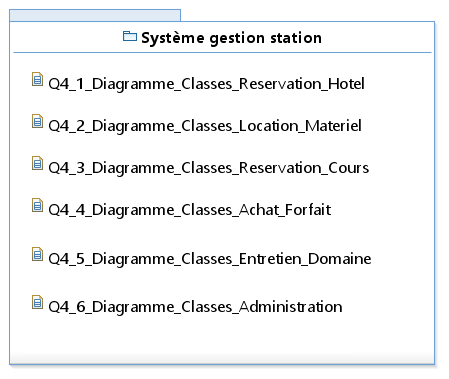
\includegraphics[width=15.5cm]{assets/pictures/Q4___Diagramme_Classes_Systeme_Gestion_Station_de_Ski.png} 
  \caption{Diagramme de classes de gestion de la station de ski}%
  %\label{Q1}
\end{figure}
\bigskip
\newpage

\section{Choix des structures de données}

\section{Algorithmes intéressants}


%%% algo balise meta pour le non-indexage d'un site
\begin{algorithm}
\caption[\emph{Balise Meta pour le non-indexage d'un site}]{\label{non_indexage}Exemple d'une balise meta pour empêcher l'indexage d'un site à la ligne 7.}
%\textbf{\textcolor{teal}{<!\,-\,- commentaire -\,->}}\\
\textbf{<!\textcolor{blue}{DOCTYPE} \textcolor{cyan}{html}>}\\
\html{}{
  \head{}{
  \smallskip
  
    \textbf{<\textcolor{blue}{title}>Exemple de non-indexage</\textcolor{blue}{title}>\\
    <\textcolor{blue}{meta} \textcolor{cyan}{charset}=\textcolor{auburn}{“UTF-8”}>\\
    \dots\\
    <\textcolor{blue}{meta} \textcolor{cyan}{name}=\textcolor{auburn}{“robots”} \textcolor{cyan}{content}=\textcolor{auburn}{“noindex”}>\\}
    \smallskip
    
  }
  \smallskip
   
  \body{}{
  \smallskip
  
  \dots\\
  \smallskip
  
  }
}
\end{algorithm}
\bigskip
